% !TEX program = pdflatex
\documentclass[12pt, a4paper]{article}

% ============================================================
% Page layout
% ============================================================
\usepackage[
  top=2.5cm, bottom=2.5cm,
  left=2.8cm, right=2.8cm,
]{geometry}
\usepackage{setspace}
\onehalfspacing

% ============================================================
% Math / Symbols
% ============================================================
\usepackage{amsmath, amssymb, bm}

% ============================================================
% Tables and floats
% ============================================================
\usepackage{graphicx}
\usepackage{booktabs}
\usepackage{multirow}
\usepackage{makecell}
\usepackage{float}
\usepackage{caption}
\captionsetup{font=small, labelfont=bf, skip=6pt}

% ============================================================
% Code listings
% ============================================================
\usepackage{listings}
\usepackage{xcolor}

\definecolor{codebg}{RGB}{248,248,248}
\definecolor{codeframe}{RGB}{200,200,200}
\definecolor{codekw}{RGB}{0,112,32}
\definecolor{codecomment}{RGB}{96,96,96}
\definecolor{codestr}{RGB}{186,33,33}

\lstset{
  backgroundcolor=\color{codebg},
  frame=single,
  rulecolor=\color{codeframe},
  basicstyle=\ttfamily\small,
  keywordstyle=\color{codekw}\bfseries,
  commentstyle=\color{codecomment}\itshape,
  stringstyle=\color{codestr},
  showstringspaces=false,
  breaklines=true,
  breakatwhitespace=true,
  tabsize=4,
  xleftmargin=1em,
  xrightmargin=0.5em,
  aboveskip=0.8em,
  belowskip=0.6em,
  numberstyle=\tiny\color{gray},
  numbers=left,
  numbersep=8pt,
  escapeinside={(*@}{@*)},
}

\lstdefinelanguage{json}{
  morestring=[b]",
  literate=
    *{:}{{{\color{black}:}}}{1}
     {,}{{{\color{black},}}}{1}
     {\{}{{{\color{black}\{}}}{1}
     {\}}{{{\color{black}\}}}}{1}
     {[}{{{\color{black}[}}}{1}
     {]}{{{\color{black}]}}}{1},
}

% ============================================================
% Hyperlinks and references
% ============================================================
\usepackage[hidelinks]{hyperref}
\usepackage[numbers, sort&compress]{natbib}

% ============================================================
% Custom commands
% ============================================================
\newcommand{\intenttype}[1]{\texttt{#1}}
\newcommand{\filepath}[1]{\texttt{#1}}
\newcommand{\yang}{\textsc{YANG}}
\newcommand{\nsp}{\textsc{NSP}}
\newcommand{\lora}{\textsc{LoRA}}
\newcommand{\fillvalues}{\texttt{fill\_values}}

% ============================================================
% TikZ diagrams
% ============================================================
\usepackage{tikz}
\usetikzlibrary{
  arrows.meta,
  positioning,
  shapes.geometric,
  shapes.multipart,
  fit,
  calc,
  backgrounds,
  decorations.pathreplacing,
}

% ============================================================
% Title
% ============================================================
\title{%
  \vspace{-1cm}
  {\LARGE\bfseries Automated Nokia NSP Network Service Intent\\[4pt]
  Generation via LoRA-Tuned Large Language Models}\\[12pt]
  {\large --- Project Proposal and Implementation Plan ---}
}
\author{%
  Liao Liu \\[3pt]
  {\small\textit{University of Ottawa}}
}
\date{\today}

% ============================================================
\begin{document}
\maketitle
\thispagestyle{empty}

% ============================================================
% Abstract
% ============================================================
\begin{abstract}
\noindent
Nokia Network Services Platform (\nsp{}) is a widely deployed network service management platform in the telecommunications industry. Its core abstraction---the \emph{intent}---is a declarative JSON object that describes the desired state of a network service. Manually authoring intent JSON is challenging due to deep field paths, low fault tolerance, and high domain-knowledge requirements. This project proposes to fine-tune the Qwen3.5-9B large language model using \lora{} (Low-Rank Adaptation) to build an end-to-end system that translates natural language network service requests into \nsp{}-compliant intent JSON. The system is designed to cover 9 intent types (epipe, tunnel, vprn, vpls, ies, etree, cpipe, evpn-epipe, evpn-vpls) and incorporates a multi-tier validation framework grounded in Nokia's official \yang{} schemas to ensure output quality. This document details the project background, available data assets, technical approach, training data synthesis strategy, and implementation plan.

\vspace{6pt}
\noindent\textbf{Keywords:} LLM fine-tuning, LoRA, network intent automation, Nokia NSP, YANG schema, structured output generation
\end{abstract}

\newpage
\tableofcontents
\newpage

% ============================================================
\section{Introduction}
% ============================================================

\subsection{Background}

Nokia \nsp{} is a unified network service orchestration platform for telecommunications operators. Its core work unit is the \emph{intent}---a declarative JSON configuration object that describes the desired state of a network service. Each intent consists of three core fields:

\begin{itemize}
  \item \textbf{intent\_type}: service type identifier (e.g., \intenttype{epipe}, \intenttype{vprn})
  \item \textbf{template\_name}: the corresponding \nsp{} template name
  \item \textbf{fill\_values}: a flat dictionary of dot-notation field paths mapped to \yang{} schema leaf nodes
\end{itemize}

\noindent
The \fillvalues{} field uses paths such as \texttt{site[0].interface[0].ipv4.primary.address}, corresponding to the hierarchical structure defined in the \yang{} schema. A typical multi-site VPRN configuration may contain 30--50 fields with path depths of 5--6 levels.

Manual authoring of \nsp{} intent JSON faces the following challenges:

\begin{enumerate}
  \item \textbf{High complexity}: deep field paths, large field counts, especially for multi-site services;
  \item \textbf{Low fault tolerance}: any path misspelling, type mismatch, or semantic conflict (e.g., missing SDP bidirectionality) results in deployment failure;
  \item \textbf{High knowledge barrier}: operators must simultaneously master \yang{} schema structures, \nsp{} API specifications, and service-specific network semantics.
\end{enumerate}

\subsection{Research Objective}

This project aims to build an end-to-end Natural Language to JSON (NL-to-JSON) automation system: operators describe network service requirements in natural language (e.g., ``Create an E-Pipe service from 192.168.0.16 to 192.168.0.37''), and the system automatically generates \nsp{}-compliant intent JSON.

\subsection{Target Intent Types}

The system is designed to support the 9 \nsp{} service intent types listed in Table~\ref{tab:intent-types}, covering L2/L3 VPN, MPLS tunneling, TDM emulation, and EVPN service categories.

\begin{table}[H]
\centering
\caption{Target 9 NSP intent types}
\label{tab:intent-types}
\small
\begin{tabular}{llll}
\toprule
\textbf{Intent Type} & \textbf{Service Category} & \textbf{Typical Scenario} & \textbf{Topology} \\
\midrule
\intenttype{epipe}       & L2 Point-to-Point & E-Line interconnect         & P2P \\
\intenttype{tunnel}      & MPLS Tunnel        & SDP tunnel establishment    & P2P \\
\intenttype{vprn}        & L3 VPN             & Multi-site IP-VPN           & Multipoint \\
\intenttype{vpls}        & L2 Multipoint      & Ethernet bridging domain    & Multipoint \\
\intenttype{ies}         & L3 Routed Access   & Internet Enhanced Service   & Single-site \\
\intenttype{etree}       & L2 Hub-Spoke       & Hub-spoke broadcast isolation & Tree \\
\intenttype{cpipe}       & TDM Emulation      & E1/T1 circuit emulation     & P2P \\
\intenttype{evpn-epipe}  & EVPN P2P           & BGP-controlled E-Line       & P2P \\
\intenttype{evpn-vpls}   & EVPN Multipoint    & BGP-controlled bridging     & Multipoint \\
\bottomrule
\end{tabular}
\end{table}

% ============================================================
\section{Available Data Assets}
\label{sec:data-assets}
% ============================================================

The project's data foundation comes from four authoritative sources, all organized and ready for training data construction.

\subsection{Nokia YANG Schemas}

We have obtained and organized the official Nokia \yang{} module files for all 9 intent types, stored under \filepath{data/yang/<intent\_type>/}. Parsing these schemas with the \texttt{pyang} library provides the following metadata for each field:

\begin{itemize}
  \item Canonical hierarchical path
  \item Base type (\texttt{int32}, \texttt{string}, \texttt{enumeration}, \texttt{boolean}, etc.)
  \item Value range constraints (e.g., \texttt{range "1..4094"} for VLAN IDs)
  \item String length constraints and regex patterns
  \item Enumeration value sets
  \item \texttt{mandatory}, \texttt{leaf-list}, \texttt{union} attributes
  \item List node key definitions and \texttt{min-elements}/\texttt{max-elements} constraints
\end{itemize}

\noindent
These schemas serve as the authoritative basis for both training data validation and model output verification.

\subsection{Nokia Canonical Payloads}

18 canonical JSON payload examples were extracted from the Nokia unified service management package (\texttt{nsp-service-mgmt-unified-25.8.3-rel.173.zip}). Their distribution is shown in Table~\ref{tab:canonical-payloads}.

\begin{table}[H]
\centering
\caption{Nokia canonical payload distribution}
\label{tab:canonical-payloads}
\small
\begin{tabular}{lcc}
\toprule
\textbf{Intent Type} & \textbf{Payload Count} & \textbf{Notes} \\
\midrule
\intenttype{vpls}        & 7 & Most comprehensive coverage \\
\intenttype{vprn}        & 3 & Includes variants with vastly different field counts \\
\intenttype{evpn-vpls}   & 3 & Covers mpls/vxlan/both modes \\
\intenttype{epipe}       & 2 & Basic dual-endpoint configurations \\
\intenttype{evpn-epipe}  & 2 & Covers mpls/vxlan modes \\
\intenttype{ies}         & 1 & Single-site routed access \\
\midrule
\intenttype{etree}       & 0 & No canonical payload in Nokia package \\
\intenttype{cpipe}       & 0 & No canonical payload in Nokia package \\
\intenttype{tunnel}      & 0 & No canonical payload in Nokia package \\
\bottomrule
\end{tabular}
\end{table}

\noindent
These payloads will be used to build a similarity-based reference validation tier (see \S\ref{sec:tier6}). Note that 3 intent types have no canonical payloads, and existing payload field coverage varies significantly (e.g., vprn payloads range from 658 to 15 fields).

\subsection{Domain Knowledge Vocabulary}

We have compiled a domain knowledge vocabulary reflecting real Nokia operator environments:

\begin{itemize}
  \item \textbf{IP address ranges}: \texttt{10.x.x.x} management network, \texttt{192.168.x.x} device interconnect
  \item \textbf{Port naming conventions}: physical ports (\texttt{1/2/c4/1}) and LAG aggregates (\texttt{lag-1} to \texttt{lag-20})
  \item \textbf{Cluster name pool}: 35 Greek letter and celestial names (Alpha, Beta, Gamma, ..., Castor)
  \item \textbf{Project name pool}: 26 operator project names (OurAI, NetFlow, CloudX, ...)
  \item \textbf{Site descriptors}: 11 site role categories (datacenter, office, branch, pop, ...)
\end{itemize}

\subsection{Nokia Service Management Guide}

Chapters 4.7--4.19 of the Nokia Service Management Guide PDF provide parameter constraint descriptions and cross-field semantic rules for each service type, which will be used to design and verify Tier 4 semantic validation rules.

% ============================================================
\section{Technical Approach}
\label{sec:approach}
% ============================================================

\subsection{Overall Architecture}

We plan to build a complete pipeline from data generation through model training, inference, and validation. Figure~\ref{fig:pipeline} illustrates the system architecture.

\begin{figure}[H]
\centering
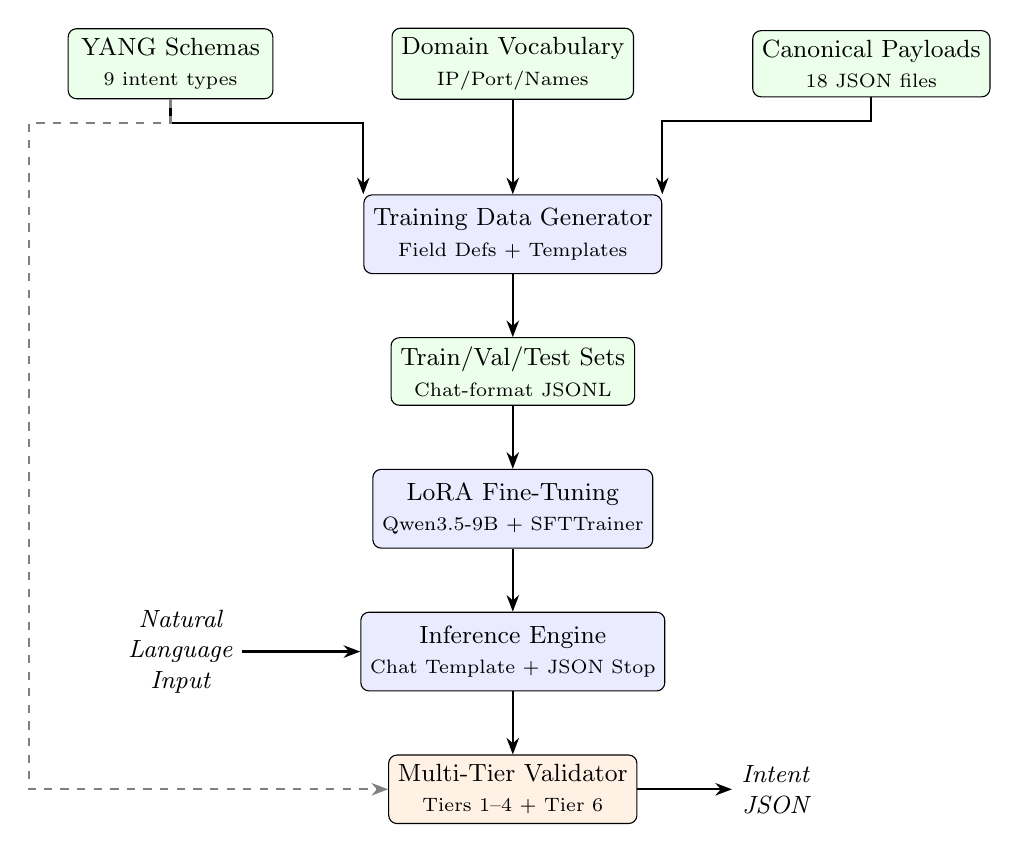
\begin{tikzpicture}[
  node distance=0.6cm and 1.2cm,
  every node/.style={font=\small},
  block/.style={
    rectangle, draw, rounded corners=3pt,
    minimum width=3.2cm, minimum height=1cm,
    fill=blue!8, align=center,
  },
  data/.style={
    rectangle, draw, rounded corners=3pt,
    minimum width=2.6cm, minimum height=0.8cm,
    fill=green!8, align=center,
  },
  valid/.style={
    rectangle, draw, rounded corners=3pt,
    minimum width=2.6cm, minimum height=0.8cm,
    fill=orange!10, align=center,
  },
  arrow/.style={-{Stealth[length=6pt]}, thick},
]
  % Data source layer
  \node[data] (yang) {YANG Schemas\\{\scriptsize 9 intent types}};
  \node[data, right=1.5cm of yang] (vocab) {Domain Vocabulary\\{\scriptsize IP/Port/Names}};
  \node[data, right=1.5cm of vocab] (canon) {Canonical Payloads\\{\scriptsize 18 JSON files}};

  % Data generation layer
  \node[block, below=1.2cm of vocab] (datagen) {Training Data Generator\\{\scriptsize Field Defs + Templates}};

  % Dataset
  \node[data, below=0.8cm of datagen] (dataset) {Train/Val/Test Sets\\{\scriptsize Chat-format JSONL}};

  % Training layer
  \node[block, below=0.8cm of dataset] (train) {LoRA Fine-Tuning\\{\scriptsize Qwen3.5-9B + SFTTrainer}};

  % Inference layer
  \node[block, below=0.8cm of train] (infer) {Inference Engine\\{\scriptsize Chat Template + JSON Stop}};

  % Validation layer
  \node[valid, below=0.8cm of infer] (validate) {Multi-Tier Validator\\{\scriptsize Tiers 1--4 + Tier 6}};

  % Arrows: data sources -> generator
  \draw[arrow] (yang.south) -- ++(0,-0.3) -| (datagen.north west);
  \draw[arrow] (vocab.south) -- (datagen.north);
  \draw[arrow] (canon.south) -- ++(0,-0.3) -| (datagen.north east);

  % Arrows: pipeline
  \draw[arrow] (datagen) -- (dataset);
  \draw[arrow] (dataset) -- (train);
  \draw[arrow] (train) -- (infer);
  \draw[arrow] (infer) -- (validate);

  % YANG to validator direct connection
  \draw[arrow, dashed, gray] (yang.south) -- ++(0,-0.3) -- ++(-1.8,0) |- (validate.west);

  % NL input
  \node[left=1.5cm of infer, align=center, font=\small\itshape] (nl) {Natural\\Language\\Input};
  \draw[arrow] (nl) -- (infer);

  % JSON output
  \node[right=1.2cm of validate, align=center, font=\small\itshape] (out) {Intent\\JSON};
  \draw[arrow] (validate) -- (out);

\end{tikzpicture}
\caption{System architecture: end-to-end pipeline from data sources to validated output}
\label{fig:pipeline}
\end{figure}

\subsection{YANG Schema Parser}
\label{sec:yang-parser}

The schema parser serves as the system's data infrastructure. We plan to use the \texttt{pyang} library to parse Nokia's \yang{} modules and build a unified \texttt{SchemaIndex}. Core design decisions include:

\begin{enumerate}
  \item \textbf{Type chain resolution}: automatically trace \texttt{import}, \texttt{uses grouping}, and \texttt{typedef} chains, resolving derived types such as \texttt{inet:ipv4-address-no-zone} to their base \texttt{string} + \texttt{pattern} forms;
  \item \textbf{Dual-mode lookup}: support both exact path matching and suffix matching---the latter handles the project convention of omitting intermediate wrapper containers (e.g., \texttt{sdp-details.});
  \item \textbf{Envelope field handling}: \nsp{}'s envelope fields (\texttt{service-name}, \texttt{intent-type}, \texttt{olc-state}, etc.) are not defined in per-intent \yang{} modules and must be registered manually.
\end{enumerate}

\noindent
Each leaf node's metadata is encapsulated as follows:

\begin{lstlisting}[language=Python, caption={LeafMeta data structure}]
@dataclass
class LeafMeta:
    path: str               # Canonical YANG path
    base_type: str          # Base type (int32/string/boolean/...)
    range_expr: str | None  # Value range constraint
    length_expr: str | None # String length constraint
    pattern_list: list[str] # Regex patterns
    enum_values: list[str]  # Enumeration value set
    mandatory: bool         # Whether mandatory
    is_leaf_list: bool      # leaf-list flag
    union_types: list       # Union member types
\end{lstlisting}

\subsection{Multi-Tier Validation Framework}
\label{sec:validation}

The validation framework is the core quality assurance mechanism. We plan to implement a five-tier progressive validation stack as illustrated in Figure~\ref{fig:validation-tiers}. Each tier runs after the previous tier passes, progressively deepening the semantic level of verification.

\begin{figure}[H]
\centering
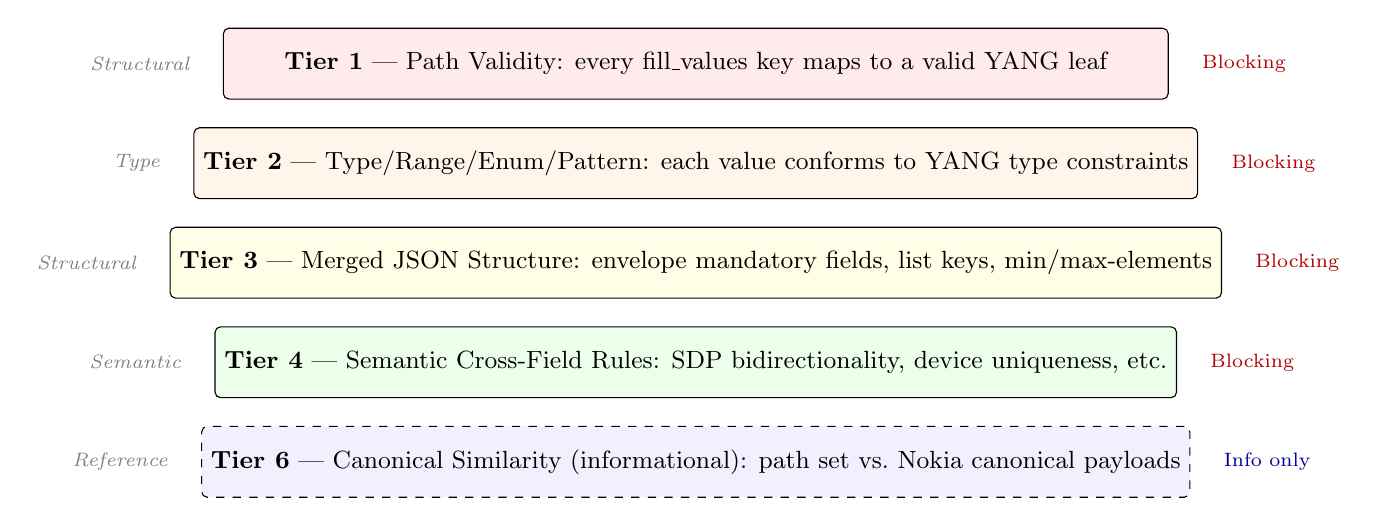
\begin{tikzpicture}[
  every node/.style={font=\small},
  tier/.style={
    rectangle, draw, rounded corners=2pt,
    minimum width=12cm, minimum height=0.9cm,
    align=center,
  },
  node distance=0.35cm,
]
  \node[tier, fill=red!8]    (t1) {\textbf{Tier 1} --- Path Validity: every fill\_values key maps to a valid YANG leaf};
  \node[tier, fill=orange!8, below=of t1] (t2) {\textbf{Tier 2} --- Type/Range/Enum/Pattern: each value conforms to YANG type constraints};
  \node[tier, fill=yellow!10, below=of t2] (t3) {\textbf{Tier 3} --- Merged JSON Structure: envelope mandatory fields, list keys, min/max-elements};
  \node[tier, fill=green!8,  below=of t3] (t4) {\textbf{Tier 4} --- Semantic Cross-Field Rules: SDP bidirectionality, device uniqueness, etc.};
  \node[tier, fill=blue!6, dashed, below=of t4] (t6) {\textbf{Tier 6} --- Canonical Similarity (informational): path set vs.\ Nokia canonical payloads};

  % Left annotations
  \node[left=0.3cm of t1, font=\scriptsize\itshape, text=gray] {Structural};
  \node[left=0.3cm of t2, font=\scriptsize\itshape, text=gray] {Type};
  \node[left=0.3cm of t3, font=\scriptsize\itshape, text=gray] {Structural};
  \node[left=0.3cm of t4, font=\scriptsize\itshape, text=gray] {Semantic};
  \node[left=0.3cm of t6, font=\scriptsize\itshape, text=gray] {Reference};

  % Right annotations
  \node[right=0.3cm of t1, font=\scriptsize, text=red!70!black] {Blocking};
  \node[right=0.3cm of t2, font=\scriptsize, text=red!70!black] {Blocking};
  \node[right=0.3cm of t3, font=\scriptsize, text=red!70!black] {Blocking};
  \node[right=0.3cm of t4, font=\scriptsize, text=red!70!black] {Blocking};
  \node[right=0.3cm of t6, font=\scriptsize, text=blue!60!black] {Info only};

\end{tikzpicture}
\caption{Five-tier progressive validation stack}
\label{fig:validation-tiers}
\end{figure}

Each tier is described in detail below.

\subsubsection{Tier 1: Path Validity}

Verifies that every key in \fillvalues{} corresponds to a valid leaf path in the \yang{} schema. The \texttt{SchemaIndex} uses suffix matching to handle abbreviated paths. For example, \texttt{sdp[0].sdp-id} is correctly identified even though its full \yang{} path is \texttt{epipe.sdp-details.sdp[0].sdp-id}.

\subsubsection{Tier 2: Type/Range/Enum/Pattern}

Performs type validation on each value:

\begin{itemize}
  \item \textbf{Integer types} (int8--int64, uint8--uint64): check base type bounds and \yang{} \texttt{range} expressions
  \item \textbf{String types}: check \texttt{length} constraints and \texttt{pattern} regexes
  \item \textbf{Enumeration types}: verify the value belongs to the valid enumeration set
  \item \textbf{Union types}: try each member type; at least one must match
  \item \textbf{Boolean types}: accept Python \texttt{bool} and string representations
\end{itemize}

\subsubsection{Tier 3: Merged JSON Structural Validation}

Runs after \fillvalues{} is merged into the full intent JSON, checking:

\begin{itemize}
  \item Root key \texttt{nsp-service-intent:intent} array exists and is non-empty
  \item Envelope mandatory fields are populated (e.g., tunnel's \texttt{name/source-ne-id/sdp-id})
  \item All \yang{} list entry key fields are present
  \item List entry counts satisfy \texttt{max-elements}/\texttt{min-elements} constraints
\end{itemize}

\subsubsection{Tier 4: Semantic Cross-Field Rules}

Validates cross-field constraints that \yang{} schemas cannot express. Table~\ref{tab:semantic-rules} lists the planned semantic rules for each intent type.

\begin{table}[H]
\centering
\caption{Tier 4 semantic rules per intent type}
\label{tab:semantic-rules}
\small
\begin{tabular}{lp{10.5cm}}
\toprule
\textbf{Intent Type} & \textbf{Semantic Rules} \\
\midrule
\intenttype{epipe} &
  SDP[0].source=site-a, SDP[1].source=site-b (bidirectionality); VLAN tags match; devices differ \\
\intenttype{tunnel} &
  source-ne-id $\neq$ destination-ne-id \\
\intenttype{vprn} &
  All site device-ids are mutually distinct; RD format is \texttt{ASN:ID} \\
\intenttype{vpls} / \intenttype{evpn-vpls} &
  Site device-ids are distinct; outer VLAN tags are consistent across all sites \\
\intenttype{etree} &
  $\geq$1 root SAP + $\geq$1 leaf SAP; site device-ids are distinct \\
\intenttype{cpipe} &
  Devices differ; time-slots match at both endpoints; vc-type in valid enum set \\
\intenttype{evpn-epipe} &
  evpn-type matches populated sub-tree (mpls or vxlan); eth-tag equals access VLAN \\
\bottomrule
\end{tabular}
\end{table}

\subsubsection{Tier 6: Canonical Payload Similarity}
\label{sec:tier6}

Compares the model output's path set against Nokia canonical payload path sets. Path normalization includes stripping wrapper containers (e.g., \texttt{*-details.}) and folding list indices to wildcards (\texttt{site[0]} $\to$ \texttt{site[*]}). This tier is informational and non-blocking, since the canonical payloads themselves are incomplete---3 intent types have no canonical payloads at all.

% ============================================================
\section{Training Data Synthesis Strategy}
\label{sec:data-generation}
% ============================================================

High-quality synthetic training data is the cornerstone of this project. We have designed a template-driven data generation pipeline whose core flow is shown in Figure~\ref{fig:datagen-flow}.

\begin{figure}[H]
\centering
\begin{tikzpicture}[
  every node/.style={font=\small},
  step/.style={
    rectangle, draw, rounded corners=3pt,
    minimum width=3cm, minimum height=0.9cm,
    fill=blue!6, align=center,
  },
  io/.style={
    trapezium, draw, trapezium left angle=70, trapezium right angle=110,
    minimum width=2.2cm, minimum height=0.7cm,
    fill=green!6, align=center, font=\small,
  },
  arrow/.style={-{Stealth[length=5pt]}, thick},
  node distance=0.5cm,
]
  \node[step] (gen) {Field Definition Generator\\{\scriptsize field\_definitions.py}};
  \node[io, right=1.5cm of gen] (fv) {fill\_values\\{\scriptsize Field dictionary}};
  \node[step, below=0.8cm of gen] (tmpl) {Template Selection\\{\scriptsize instruction\_templates.py}};
  \node[io, right=1.5cm of tmpl] (inst) {NL Instruction\\{\scriptsize User message}};
  \node[step, below=0.8cm of tmpl] (valid) {Sample Validation\\{\scriptsize Tiers 1+2+4}};
  \node[step, below=0.8cm of valid] (assemble) {Chat Format Assembly\\{\scriptsize (system, user, assistant)}};
  \node[io, below=0.8cm of assemble] (jsonl) {JSONL Output\\{\scriptsize train/val/test}};

  \draw[arrow] (gen) -- (fv);
  \draw[arrow] (fv.south) -- ++(0,-0.25) -| (tmpl.east);
  \draw[arrow] (tmpl) -- (inst);
  \draw[arrow] (gen.south) -- (tmpl.north);
  \draw[arrow] (tmpl) -- (valid);
  \draw[arrow] (fv.south) -- ++(0,-0.25) -- ++(2.5,0) |- (valid.east);
  \draw[arrow] (valid) -- node[right, font=\scriptsize] {Pass} (assemble);
  \draw[arrow] (assemble) -- (jsonl);
\end{tikzpicture}
\caption{Training data generation pipeline}
\label{fig:datagen-flow}
\end{figure}

\subsection{Field Definition Generators}

Each intent type has a dedicated generator function that produces a semantically consistent \fillvalues{} dictionary. A unified dispatcher routes to the appropriate generator:

\begin{lstlisting}[language=Python, caption={Unified dispatch interface}]
def generate_intent_values(intent_type: str, **opts) -> dict:
    """Route to per-intent generator, return fill_values dict."""
\end{lstlisting}

\noindent
Generators must satisfy the following constraints:

\begin{itemize}
  \item Produced \fillvalues{} must pass Tier 1+2 validation (correct paths and types)
  \item Inter-field semantic relationships must satisfy Tier 4 rules (e.g., epipe SDP bidirectionality)
  \item Domain knowledge vocabulary must be used for realistic IP, port, and name values
\end{itemize}

\subsubsection{Traditional Generators}

For epipe, tunnel, vprn, vpls, ies, etree, and cpipe, generators use internal random sampling to produce field values. For example:

\begin{itemize}
  \item \texttt{random\_device\_ip()} samples from the \texttt{192.168.x.x} range
  \item \texttt{random\_port\_id()} generates Nokia port formats (\texttt{1/2/c4/1} or \texttt{lag-12})
  \item \texttt{derive\_sdp\_id(src\_ip, dst\_ip)} deterministically derives the SDP ID from IP addresses
\end{itemize}

These random values simultaneously populate instruction template placeholders, ensuring the model can derive all output information from the input.

\subsubsection{Pure Function Generators --- A Key Design Innovation}
\label{sec:pure-function}

For EVPN types (evpn-epipe, evpn-vpls), we plan to employ a \textbf{pure function generator} design. The core contract states:

\begin{quote}
\itshape
Every field value returned by the generator must satisfy one of three conditions:\\
(a) it is a direct copy of an instruction-visible parameter;\\
(b) it is a fixed constant for that intent type (e.g., mtu=1500);\\
(c) it is a deterministic function of instruction-visible parameters (e.g., RD = ``65000:\{ne\_service\_id\}'').
\end{quote}

\noindent
The motivation is that if \fillvalues{} contains random values invisible to the instruction template, the model faces an \textbf{unlearnable task}---no amount of training can push accuracy for those fields beyond the random baseline.

The implementation separates random sampling from deterministic generation into two steps:

\begin{lstlisting}[language=Python, caption={Pure function generator: two-step separation}]
# Step 1: Centralized random sampling for instruction-visible args
args = _roll_evpn_epipe_args()

# Step 2: Pure function generation (no internal random calls)
fill_values = generate_evpn_epipe_values(**args)

# Step 3: Same args drive the instruction template
instruction = template.format(**args)
\end{lstlisting}

\noindent
Planned deterministic derivation rules (following Nokia operator practice) are shown in Table~\ref{tab:deterministic-rules}.

\begin{table}[H]
\centering
\caption{EVPN pure function generator deterministic derivation rules}
\label{tab:deterministic-rules}
\small
\begin{tabular}{lll}
\toprule
\textbf{Field} & \textbf{Derivation Rule} & \textbf{Type} \\
\midrule
RD / RT            & \texttt{"65000:\{ne\_service\_id\}"} & Deterministic function \\
VNI                & \texttt{ne\_service\_id}             & Direct copy \\
vsi-import         & \texttt{["\{service\_name\}-import"]} & Deterministic function \\
vsi-export         & \texttt{["\{service\_name\}-export"]} & Deterministic function \\
eth-tag            & \texttt{vlan}                        & Direct copy \\
mtu                & 1500                                  & Constant \\
ecmp               & 4                                     & Constant \\
\bottomrule
\end{tabular}
\end{table}

\subsection{Instruction Template Design}

Each intent type will have 10--15 natural language templates covering four linguistic styles:

\begin{enumerate}
  \item \textbf{Formal/Complete}: all parameters explicitly stated
  \item \textbf{Conversational}: natural question/request tone
  \item \textbf{Terse/Operational}: compact key=value format
  \item \textbf{Contextual}: includes project/scenario background
\end{enumerate}

\noindent
Example templates for \intenttype{epipe}:

\begin{lstlisting}[language={}, caption={Epipe instruction template examples (three styles)}, numbers=none]
(*@\textit{// Formal style}@*)
"Create an E-Pipe service named '{service_name}' for
customer {customer_id}. Connect device {site_a_device}
on port {site_a_port} to device {site_b_device}..."

(*@\textit{// Conversational style}@*)
"I need a point-to-point Ethernet connection between
{site_a_device} and {site_b_device}. The service is
for customer {customer_id}, called '{service_name}'..."

(*@\textit{// Terse style}@*)
"Deploy epipe: {service_name}, cust={customer_id},
svc-id={ne_service_id}, mtu={mtu}, ..."
\end{lstlisting}

\noindent
Diverse template styles enable the model to generalize across different phrasings of the same network intent.

\subsection{Data Format and Scale Planning}

Each sample uses the OpenAI chat format triplet (\texttt{system}, \texttt{user}, \texttt{assistant}):

\begin{lstlisting}[language=json, caption={Training sample format example}]
{
  "messages": [
    {"role": "system",    "content": "You are an NSP intent..."},
    {"role": "user",      "content": "Create an E-Pipe..."},
    {"role": "assistant", "content": "{\"intent_type\":\"epipe\",...}"}
  ]
}
\end{lstlisting}

\noindent
Planned dataset scale:

\begin{table}[H]
\centering
\caption{Dataset split plan}
\label{tab:data-split}
\small
\begin{tabular}{lcl}
\toprule
\textbf{Split} & \textbf{Samples} & \textbf{Purpose} \\
\midrule
Training (train.jsonl) & $\sim$2640 & SFT fine-tuning \\
Validation (val.jsonl)   & $\sim$330  & eval\_loss monitoring during training \\
Test (test.jsonl)  & $\sim$330  & Final model evaluation \\
Golden Tests (golden\_tests.jsonl) & $\sim$11 & Hand-crafted edge cases \\
\midrule
\textbf{Total} & $\sim$\textbf{3311} & --- \\
\bottomrule
\end{tabular}
\end{table}

\noindent
The 9 intent types are uniformly distributed, with approximately 367 samples each. The golden test set will be hand-crafted to cover multi-site configurations, boundary values, and easily confused types.

\subsection{Data Quality Assurance}

Every generated training sample will pass the validator's Tier 1+2+4 checks before being written to JSONL, ensuring the training data itself is \yang{}-compliant and semantically correct.

% ============================================================
\section{Model Training Plan}
\label{sec:training}
% ============================================================

\subsection{Base Model Selection}

We select \textbf{Qwen3.5-9B} (Qwen/Qwen3.5-9B) as the base model for the following reasons:

\begin{itemize}
  \item 9 billion parameters with strong code generation and structured output capabilities
  \item 32K context window, sufficient for complex multi-site intent outputs
  \item Native bilingual (Chinese/English) support for future extension
  \item Built-in \texttt{<think>} tag in the chat template that requires alignment between training and inference (see \S\ref{sec:chat-template})
\end{itemize}

\subsection{LoRA Fine-Tuning Configuration}

We adopt \lora{} (Low-Rank Adaptation) for parameter-efficient fine-tuning, training only $\sim$0.65\% of parameters:

\begin{table}[H]
\centering
\caption{LoRA hyperparameter configuration}
\label{tab:lora-config}
\small
\begin{tabular}{ll}
\toprule
\textbf{Parameter} & \textbf{Value} \\
\midrule
Rank ($r$)                & 32 \\
Scaling factor ($\alpha$) & 64 ($\alpha/r = 2.0$) \\
Target modules           & q\_proj, k\_proj, v\_proj, o\_proj, gate\_proj, up\_proj, down\_proj \\
Dropout                  & 0.05 \\
Trainable parameters     & $\sim$58M / 9B (0.65\%) \\
\bottomrule
\end{tabular}
\end{table}

\noindent
Target modules cover all 4 attention projection matrices (Q/K/V/O) and 3 FFN matrices (gate/up/down), totaling 7 module types.

\subsection{Training Hyperparameters}

\begin{table}[H]
\centering
\caption{SFT training hyperparameters}
\label{tab:sft-config}
\small
\begin{tabular}{ll}
\toprule
\textbf{Parameter} & \textbf{Value} \\
\midrule
Training epochs                & 5 \\
Per-device batch size          & 2 \\
Gradient accumulation steps    & 8 \\
Effective batch size           & $2 \times 8 \times 2\text{ GPUs} = 32$ \\
Learning rate                  & $2 \times 10^{-4}$ \\
LR scheduler                  & Cosine \\
Warmup ratio                  & 0.05 \\
Weight decay                  & 0.01 \\
Max gradient norm             & 1.0 \\
Max sequence length           & 8192 tokens \\
Precision                     & BF16 \\
Evaluation frequency          & Every 50 steps \\
\bottomrule
\end{tabular}
\end{table}

\subsection{Hardware Environment}

\begin{itemize}
  \item 2 $\times$ NVIDIA RTX 6000 Ada Generation (50.9\,GB VRAM)
  \item Parallelism: DDP (Distributed Data Parallel) via the Accelerate library
  \item Each GPU loads the full BF16 model ($\sim$18\,GB), no quantization needed
  \item Gradient checkpointing enabled to conserve VRAM
\end{itemize}

\subsection{Chat Template Alignment Strategy}
\label{sec:chat-template}

Qwen3.5's chat template automatically inserts a \texttt{<think>} block when rendering assistant messages. After template rendering, the training data byte sequence is:

\begin{lstlisting}[language={}, numbers=none]
<|im_start|>assistant
<think>

</think>

{"intent_type": ...}<|im_end|>
\end{lstlisting}

\noindent
The \texttt{<think>} block is always empty and closed. At inference time, the byte sequence at the generation start position must be \textbf{byte-identical} to training. We plan to achieve this alignment by setting \texttt{enable\_thinking=False}:

\begin{lstlisting}[language=Python, caption={Chat template alignment at inference}]
prompt = tokenizer.apply_chat_template(
    messages,
    tokenize=False,
    add_generation_prompt=True,
    enable_thinking=False,  # (*@Key: byte-level alignment@*)
)
\end{lstlisting}

% ============================================================
\section{Inference and Evaluation Plan}
\label{sec:eval}
% ============================================================

\subsection{Inference Engine Design}

The inference module plans to implement the following technical features:

\begin{enumerate}
  \item \textbf{JSON stopping criteria}: a custom \texttt{StoppingCriteria} tracking brace nesting count, stopping generation immediately when the count returns to zero to avoid unnecessary token waste;
  \item \textbf{Multi-strategy JSON extraction}: try whole-text parsing, fenced code block extraction, and greedy brace matching in priority order;
  \item \textbf{End-to-end pipeline}: chain inference, JSON extraction, \fillvalues{} merging, and four-tier validation.
\end{enumerate}

\subsection{Evaluation Metrics}

The evaluation module will run full inference + validation for each test sample, reporting the metrics listed in Table~\ref{tab:eval-metrics}.

\begin{table}[H]
\centering
\caption{Evaluation metrics}
\label{tab:eval-metrics}
\small
\begin{tabular}{lp{9.5cm}}
\toprule
\textbf{Metric} & \textbf{Definition} \\
\midrule
JSON Valid Rate       & Fraction of outputs parseable as valid JSON \\
Intent Type Accuracy  & Intent type prediction accuracy \\
Field Recall          & $|\text{predicted} \cap \text{ground truth}| \;/\; |\text{ground truth}|$ \\
Field Precision       & $|\text{predicted} \cap \text{ground truth}| \;/\; |\text{predicted}|$ \\
Value Accuracy        & Fraction of matched fields with exact value match \\
Tier 1+2 Valid        & Path and type validation pass rate \\
Tier 3 Valid          & Merged structure validation pass rate \\
Tier 4 Valid          & Semantic validation pass rate \\
All Tiers Valid       & Pass rate across all four tiers simultaneously \\
Tier 6 Recognition    & Canonical payload path coverage (informational) \\
\bottomrule
\end{tabular}
\end{table}

\noindent
Evaluation will include per-intent-type breakdowns to identify weak points. Incremental checkpoint files ensure that inference results are not lost if the process is interrupted.

\subsection{Target Metrics}

Based on task characteristics and related work, we set the following targets:

\begin{itemize}
  \item JSON Valid Rate $\geq$ 95\%
  \item Value Accuracy $\geq$ 95\%
  \item All Tiers Valid $\geq$ 95\%
  \item Each individual intent type should meet the above thresholds
\end{itemize}

% ============================================================
\section{Implementation Plan and Milestones}
\label{sec:milestones}
% ============================================================

The project proceeds through five milestones, each with defined deliverables and acceptance criteria.

\begin{table}[H]
\centering
\caption{Project milestone plan}
\label{tab:milestones}
\small
\begin{tabular}{clp{7cm}l}
\toprule
\textbf{Milestone} & \textbf{Name} & \textbf{Objective} & \textbf{Deliverables} \\
\midrule
M1 & YANG Validator &
  Implement schema parser and Tier 1+2 validation for 3 base types (epipe, tunnel, vprn) &
  Validator code + unit tests \\
\addlinespace
M2 & Path Unification &
  Replace hand-written path mappings with YANG-driven resolution; verify equivalence &
  Equivalence regression tests \\
\addlinespace
M2.5 & Inference Alignment &
  Resolve chat template \texttt{<think>} alignment; fix inference max\_tokens &
  Inference code + fix report \\
\addlinespace
M3 & Horizontal Expansion &
  Expand from 3 to 9 intent types; implement field definitions, templates, and Tier 4 rules per type &
  Complete 9-type dataset \\
\addlinespace
M3.5 & Quality Sprint &
  Pure function generators (EVPN); E-Tree SDP semantic fix; canonical payload validation tier &
  Final training + evaluation \\
\bottomrule
\end{tabular}
\end{table}

% ============================================================
\section{Anticipated Challenges and Mitigation Strategies}
\label{sec:challenges}
% ============================================================

\subsection{Chat Template Train-Inference Mismatch}

Qwen3.5's \texttt{<think>} tag may be in inconsistent states between training and inference, causing output degradation. \textbf{Mitigation}: use \texttt{enable\_thinking=False} at inference to ensure byte-level alignment.

\subsection{Information Leakage of Unlearnable Fields}

If \fillvalues{} contains random values invisible to the instruction, the model cannot learn those fields. \textbf{Mitigation}: adopt the pure function generator contract for complex types like EVPN (\S\ref{sec:pure-function}), enforced by determinism tests.

\subsection{Sequence Length for Complex Topologies}

Multi-site configurations (e.g., etree with 5 sites + SDP mesh) may produce token sequences exceeding max\_length. \textbf{Mitigation}: set max\_length to 8192 (well within Qwen3.5's 32K context window) and verify all sample lengths with a dry-run script before training.

\subsection{E-Tree Topology Semantics}

E-Tree services require that leaf nodes cannot communicate with each other. Naively reusing VPLS's full-mesh SDP topology would violate this semantic. \textbf{Mitigation}: generate only root-leaf bidirectional SDPs with a fixed 1-root + N-leaf topology.

\subsection{Incomplete Canonical Payload Coverage}

etree, cpipe, and tunnel have no canonical payloads in the Nokia package, so Tier 6 cannot provide references for these types. \textbf{Mitigation}: define Tier 6 as informational (non-blocking) and ensure thorough structural and semantic checking in Tiers 1--4.

% ============================================================
\section{Limitations}
\label{sec:limitations}
% ============================================================

\begin{enumerate}
  \item \textbf{Offline validation as a structural lower bound}: Tier 1--4 passing only means the output is structurally consistent with the \yang{} schema. \nsp{}'s server-side JavaScript mapping engine performs additional transformations and validations---\texttt{valid=True} does not guarantee \nsp{} will accept the intent.
  \item \textbf{Same-distribution test set}: The test set is produced by the same generator, and cannot evaluate the model's generalization to out-of-distribution instructions.
  \item \textbf{No device intent coverage}: Nokia \nsp{} contains 181 device-intent types; this project covers only 9 service-intent types.
\end{enumerate}

% ============================================================
\section{Future Work}
% ============================================================

\begin{itemize}
  \item \textbf{Device intent type expansion}: extend to 181 device-intent types; the \yang{} schema directory structure already accommodates this.
  \item \textbf{Live deployment validation}: connect to a real \nsp{} instance to verify generated intents' deployment acceptance and success rates.
  \item \textbf{CLI generation}: leverage \texttt{payload*.cli.txt} files in the Nokia package to train JSON-to-CLI or NL-to-CLI capabilities.
  \item \textbf{Composite intents}: explore compound intents (combining multiple service types) and redundancy intents (active-standby configurations).
\end{itemize}

% ============================================================
% References
% ============================================================
\bibliographystyle{plainnat}
\begin{thebibliography}{9}

\bibitem{hu2022lora}
E.~J.~Hu, Y.~Shen, P.~Wallis, Z.~Allen-Zhu, Y.~Li, S.~Wang, L.~Wang, and
  W.~Chen.
\newblock Lo{RA}: Low-rank adaptation of large language models.
\newblock In {\em ICLR}, 2022.

\bibitem{qwen2025}
Qwen Team.
\newblock Qwen3 technical report.
\newblock {\em arXiv preprint arXiv:2505.09388}, 2025.

\bibitem{rfc7950}
M.~Bjorklund.
\newblock The {YANG} 1.1 data modeling language.
\newblock RFC 7950, IETF, August 2016.

\bibitem{nokia-nsp}
Nokia.
\newblock {\em Network Services Platform --- Service Management Guide}, release
  25.8 edition, 2025.

\bibitem{trl}
L.~von Werra, Y.~Belkada, L.~Tunstall, E.~Beeching, T.~Thrush, N.~Lambert,
  and S.~Huang.
\newblock {TRL}: Transformer Reinforcement Learning.
\newblock \url{https://github.com/huggingface/trl}, 2020.

\bibitem{peft}
S.~Mangrulkar, S.~Gugger, L.~Debut, Y.~Belkada, S.~Paul, and B.~Bossan.
\newblock {PEFT}: State-of-the-art parameter-efficient fine-tuning methods.
\newblock \url{https://github.com/huggingface/peft}, 2022.

\bibitem{pyang}
M.~Bjorklund.
\newblock pyang --- {YANG} validator and converter.
\newblock \url{https://github.com/mbj4668/pyang}, 2023.

\end{thebibliography}

\end{document}
